\subsection{RQ2: Gradients and training}
\label{sec:gradients}
\begin{figure*}[!t]
\centering
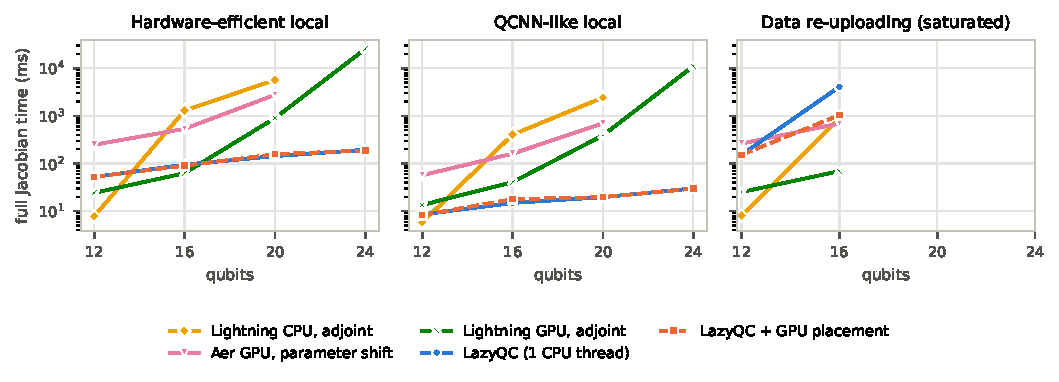
\includegraphics[width=\textwidth]{figures/gradient_scaling.pdf}
\caption{Time to obtain the full Jacobian of all $n$ outputs with respect to every trainable rotation, median per case and geometric mean over two seeds. The planner evaluates the base program and every $\pm\pi/2$ shift as one batch; Aer GPU runs every shifted circuit; Lightning uses adjoint differentiation. At 24 qubits the adjoint Jacobian with all observables exceeded GPU memory and was computed in chunks of eight observables. The saturated family was evaluated up to 16 qubits. Lower is better.}
\label{fig:gradients}
\end{figure*}

\begin{table*}[!t]
\caption{Full Jacobians: Trainable Rotations $P$, Distinct Tasks of the Planner, Structurally Zero Derivatives, and Median Time in Milliseconds per Method.}
\label{tab:jacobian}
\centering
\footnotesize
\setlength{\tabcolsep}{4pt}
\begin{tabular}{lrrrrrrrr}
\toprule
Family & $n$ & $P$ & Tasks & Zeros (\%) & LazyQC & Aer shift & L.\ GPU adj. & L.\ CPU adj.\\
\midrule
Re-uploading & 12 & 48 & 97 & 10 & 152 & 263 & 25 & 8.0\\
Re-uploading & 16 & 64 & 129 & 10 & 1{,}039 & 694 & 69 & 909\\
Hardware-eff. & 12 & 48 & 290 & 51 & 53 & 247 & 24 & 7.8\\
Hardware-eff. & 16 & 64 & 404 & 61 & 90 & 535 & 63 & 1{,}290\\
Hardware-eff. & 20 & 80 & 518 & 68 & 157 & 2{,}761 & 896 & 5{,}656\\
Hardware-eff. & 24 & 96 & 632 & 73 & 187 & n/a & 25{,}310 & n/a\\
QCNN-like & 12 & 22 & 102 & 74 & 8.3 & 57 & 13 & 5.8\\
QCNN-like & 16 & 32 & 158 & 80 & 18 & 161 & 41 & 403\\
QCNN-like & 20 & 38 & 181 & 84 & 20 & 701 & 390 & 2{,}422\\
QCNN-like & 24 & 48 & 237 & 86 & 30 & n/a & 11{,}048 & n/a\\
\bottomrule
\end{tabular}

\end{table*}

Gradient workloads multiply the number of requested circuits. Under the parameter-shift rule of Eq.~\eqref{eq:shift}, one Jacobian with respect to $P$ rotation occurrences requires the base circuit and $2P$ shifted ones, each with all $K$ outputs. They are also where a simulator has its strongest alternative: adjoint differentiation obtains all derivatives of an observable from about two passes over the state~\cite{jones2020adjoint}. We therefore compare the planner's shift-rule Jacobian with Aer GPU running every shifted circuit and with Lightning's adjoint method on the GPU and on the CPU (Fig.~\ref{fig:gradients} and Table~\ref{tab:jacobian}).

The object in this subsection is explicit: a full $K\times P$ Jacobian, with $K=n$ outputs and $(2P+1)K$ raw expectation requests. Table~\ref{tab:jacobian} reports $P$, the planner's distinct tasks, structurally zero entries and absolute times; Fig.~\ref{fig:gradients} compares methods computing that same object. Full Jacobians are useful for multi-output sensitivity, kernel construction and higher-order training methods, but are not required for an ordinary scalar-loss gradient step. The adjoint baseline is therefore configured to return the full Jacobian, including observable chunking when memory requires it; the cheaper scalar-loss vector-Jacobian product is evaluated separately below. The per-request Qiskit LightCone baseline for the raw expectation batch is reported in Table~\ref{tab:lightcone-ablation}.

\textbf{Shift rules meet cones.} The planner receives the $(2P+1)K$ requests of one Jacobian as a single batch. A shift that falls outside an output's cone leaves that output's cone circuit unchanged, so grouping evaluates it once together with the unshifted circuit, and the corresponding derivative comes out exactly zero without any special handling. These structural zeros are common: they are 51 to 73\% of the hardware-efficient Jacobian entries and 74 to 86\% of the QCNN-like ones. They rely on every rotation having its own parameter. When one parameter is shared by all rotations of a layer, a derivative is zero only if no occurrence of that parameter lies in the cone, and in a control at 8 and 12 qubits and depths two and four the median fraction fell from 0.49 to 0 on the hardware-efficient family and from 0.71 to 0.38 on the QCNN-like one. The planner does not run fewer circuits than direct parameter shift (632 tasks against 193 dense evolutions for the 24-qubit hardware-efficient Jacobian), but each of its tasks has at most 10 qubits, and structure-keyed analysis keeps planning at 44\,ms for 4,632 requests.

\textbf{Against adjoint differentiation.} At 12 qubits, CPU adjoint differentiation is the fastest way to obtain a Jacobian (7.8 against 53\,ms for the planner on the hardware-efficient family), and at 16 qubits GPU adjoint still leads on that family (63 against 90\,ms), while the planner is already 2.3 times faster on the QCNN-like one. From 20 qubits on the order reverses. The planner obtains the hardware-efficient Jacobian in 0.15\,s, against 0.90\,s for GPU adjoint and 2.8\,s for GPU parameter shift, and the QCNN-like one in 20\,ms against 0.39\,s. At 24 qubits the adjoint Jacobian with all 24 observables ran out of the GPU's 8\,GB, because the adjoint method keeps one state per observable during the backward pass. Computed in chunks of eight observables, it took 25\,s for the hardware-efficient family and 11\,s for the QCNN-like one, about 135 and 370 times the planner's 0.19 and 0.03\,s. Parameter shift on the GPU was the slowest option at every width, as expected from its $2P+1$ dense evolutions. For the saturated family the picture inverts: only 10\% of the derivatives are structural zeros, the planner evaluates all $2P+1$ circuits densely, and GPU adjoint is 15 times faster than the planner with GPU placement at 16 qubits. Cones help gradients exactly where they help forward passes.

\begin{table}[!t]
\caption{Ten Measured Gradient-Descent Steps on the Hardware-Efficient Family with $Z$ on Every Wire, Including Program or Tape Construction at Every Step.}
\label{tab:training}
\centering
\footnotesize
\begin{tabular}{rlrrr}
\toprule
$n$ & Method & Total (s) & Step (ms) & Final loss\\
\midrule
16 & Aer GPU, shift rule & 9.14 & 913 & 0.0841\\
16 & LazyQC, shift rule & 1.21 & 124 & 0.0841\\
16 & Lightning GPU, adjoint & 0.24 & 24 & 0.0841\\
20 & LazyQC, shift rule & 1.80 & 179 & 0.0760\\
20 & Lightning GPU, adjoint & 1.37 & 137 & 0.0760\\
24 & LazyQC, shift rule & 2.46 & 246 & 0.0909\\
24 & Lightning GPU, adjoint & 33.55 & 3355 & 0.0909\\
\bottomrule
\end{tabular}

\end{table}

\textbf{Training loops.} A training step does not need the full Jacobian, only the gradient of a scalar loss, which adjoint differentiation obtains as a single vector-Jacobian product. Table~\ref{tab:training} reports ten measured gradient-descent steps of a mean-squared loss over all outputs, each step paying for building the shifted programs or the tape, planning or executing, and updating the parameters. All methods follow the same loss trajectory, within $10^{-16}$ at every step. Here the planner competes with a cheaper quantity than before, and it loses at small widths: GPU adjoint is 5.0 times faster at 16 qubits and 1.3 times at 20. At 24 qubits the planner completes the ten steps in 2.5\,s against 33.6\,s, 13.6 times faster, because its steps grow with the number of outputs while every adjoint step doubles with each added qubit.
